%============================ MAIN DOCUMENT ================================
\PassOptionsToPackage{table}{xcolor}
\documentclass[
  a4paper,
  bibliography=totoc,
  listof=totoc,
  invert-title,
  titleimage-ratio=13
]{bfhpub}

\usepackage[french,english,main=ngerman]{babel}  % https://www.namsu.de/Extra/pakete/Babel.html
\LoadBFHModule{listings,terminal,boxes}

%---------------------------------------------------------------------------
% Documents paths
%---------------------------------------------------------------------------
\makeatletter
\def\input@path{{content/}}
\makeatother

%---------------------------------------------------------------------------
% Hyperref Package (Create links in a pdf)
%---------------------------------------------------------------------------
\usepackage[
	,bookmarks
	,plainpages=false
	,pdfpagelabels
    ,pdfusetitle
	,backref = {false}          % No index backreference
	,colorlinks = {true}        % Color links in a PDF
	,hypertexnames = {true}     % no failures "same page(i)"
	,bookmarksopen = {true}     % opens the bar on the left side
	,bookmarksopenlevel = {0}   % depth of opened bookmarks
	,linkcolor=.
	,filecolor=.
	,urlcolor=.
	,citecolor=.
]{hyperref}

%---------------------------------------------------------------------------
% Base packages
%---------------------------------------------------------------------------
% Include Packages
\usepackage{amsmath}          % various features to facilitate writing math formulas
\usepackage{amsthm}           % enhanced version of latex's newtheorem
\usepackage{amsfonts}         % set of miscellaneous TeX fonts that augment the standard CM
\usepackage{amssymb}          % mathematical special characters

\usepackage{siunitx}

\usepackage{graphicx}         % integration of images
\usepackage{float}            % floating objects

\usepackage{caption}          % for captions of figures and tables
\usepackage{subcaption}       % for subcaptions in subfigures
\usepackage{wrapfig}

\usepackage{exscale}          % mathematical size corresponds to textsize
\usepackage{multirow}         % multirow emables combining rows in tables
\usepackage{multicol}

\usepackage{longtable}
\usepackage{adjustbox}

%---------------------------------------------------------------------------
% Graphics paths
%---------------------------------------------------------------------------
\graphicspath{{pictures/}{figures/}}

%---------------------------------------------------------------------------
% Blind text -> for dummy text
%---------------------------------------------------------------------------
\usepackage{blindtext}    
\usepackage{letltxmacro}   
\LetLtxMacro{\blindtextblindtext}{\blindtext}

\RenewDocumentCommand{\blindtext}{O{\value{blindtext}}}{
	\begingroup\color{BFH-Gray}\blindtextblindtext[#1]\endgroup
}

%---------------------------------------------------------------------------
% Bibliography Package
%---------------------------------------------------------------------------
\usepackage{csquotes}
\usepackage[backend=biber,style=ieee]{biblatex}
\addbibresource{references.bib}

%---------------------------------------------------------------------------
% Glossary Package
%---------------------------------------------------------------------------
\usepackage[nonumberlist, acronym]{glossaries-extra}
\setabbreviationstyle[acronym]{long-short}
\makeglossaries
%----------------  Glossary Entries  ---------------------------------------
\newglossaryentry{latex}{
    name=LaTeX,
    description={Ein Textsatzsystem für wissenschaftliche Dokumente}
}

\newglossaryentry{bfh}{
    name=BFH,
    description={Berner Fachhochschule}
}

%----------------  Acronyms  -----------------------------------------------
\newacronym{ai}{AI}{Artificial Intelligence}
\newacronym{ml}{ML}{Machine Learning}

%---------------------------------------------------------------------------
% Makeindex Package
%---------------------------------------------------------------------------
\usepackage{makeidx}
\makeindex

\begin{document}

%------------ START FRONT PART ---------------------------------------------------------------------------------------------------------------------------
\frontmatter % Nummerierung der Seiten in römischen Zahlen

%----------------  BFH tile page   -----------------------------------------
  \title{Projekt 4: Kombinatorische Logik}
  \subtitle{BTE5213 Laborprojekte, Herbstsemester 2025/2026\\Protokoll}
  \author{Janis Aebischer \and Simon Eisele}
  \department{Technik und Informatik}
  \institute{Elektrotechnik und Informationstechnologie}
  \version{1.0}
  \titlegraphic{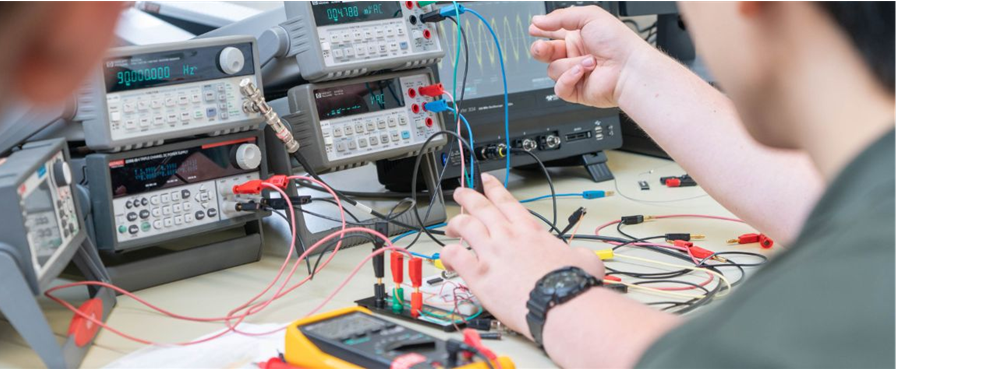
\includegraphics{Bild1.png}}
  \partnerlogo{
\includegraphics[height=\height]{bfh-logo.pdf}}

  \maketitle

%----------------  Abstract   ----------------------------------------------
\section*{Abstract}
\addcontentsline{toc}{section}{Abstract}
One-paragraph summary of the entire study – typically no more than 250 words in length (and in many cases it is well shorter than that), the Abstract provides an overview of the study.
\thispagestyle{plain}

%----------------  Table of contents   -------------------------------------
\clearpage
\tableofcontents

%------------ START MAIN PART ----------------------------------------------------------------------------------------------------------------------------
\mainmatter % Beginn mit normaler Nummerierung der Seiten

%----------------  Introduction   ------------------------------------------
\clearpage
\section{Einleitung}
\section{Introduction}

What is the topic and why is it worth studying? – the first major section of text in the paper, the Introduction commonly describes the topic under investigation, summarizes or discusses relevant prior research (for related details, please see the Writing Literature Reviews section of this website), identifies unresolved issues that the current research will address, and provides an overview of the research that is to be described in greater detail in the sections to follow.

%----------------  Methods   -----------------------------------------------
\clearpage
\section{Methoden und Materialien}
Das Ziel des Abschnitts «Methoden und Materialien» ist es, dem Leser die Gelegenheit zu bieten, alle Phasen des Versuchs reproduzieren zu können.

\begin{itemize}
    \item[-] Beschreiben Sie Ihre Herangehensweise inklusive Arbeitsaufteilung und den Ablauf des Versuchs. Zitieren Sie dabei jeweils zusätzlich verwendete Ressourcen [8] und referenzieren Sie diese im Literaturverzeichnis.
    \item[-] Listen Sie alle genutzten Geräte [9] und Software [2] und referenzieren Sie jeweils deren Dokumentation im Literaturverzeichnis.
\end{itemize}

\gls{latex} wird oft für wissenschaftliche Arbeiten genutzt. \gls{ai} ist ein Teilbereich von \gls{ml}. Zweite Verwendung von \gls{ai} und \gls{ml}. Test \gls{bfh}.


Hier wird ein Werk zitiert.\cite{EinsteinCoefficientsSpringerLink}

Hie rwird ein weiteres Werk zitiert.\cite{5GrundlagenFur2025}

% ----------------- Bilder -----------------
\begin{figure}[H]
    \centering
    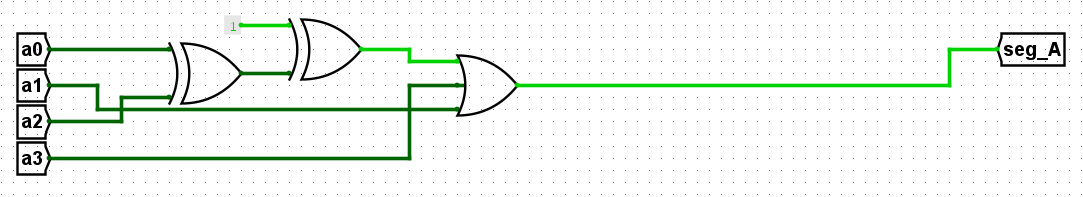
\includegraphics[width=1\textwidth]{segment_A.png}
    \caption{Logikschaltung Segment A}
    \label{fig:segment_A}
\end{figure}

Die Logikschaltung zum Segment A wurde wie in Abbildung~\ref{fig:segment_A} gezeigt aufgebaut.

\begin{figure}[H]
    \centering
    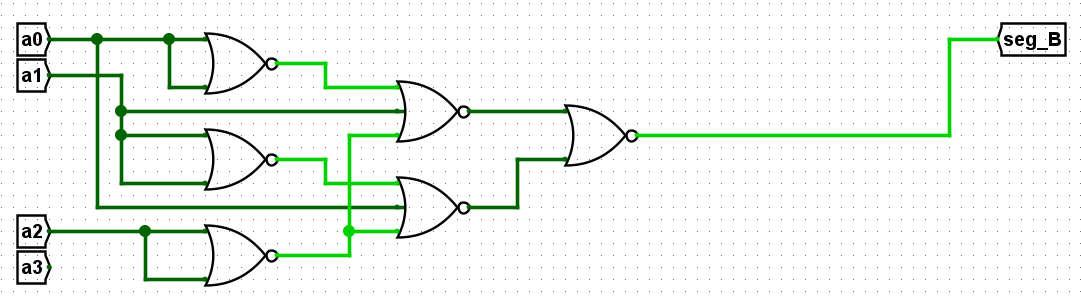
\includegraphics[width=1\textwidth]{segment_B.png}
    \caption{Logikschaltung Segment B}
    \label{fig:segment_B}
\end{figure}

Die Logikschaltung zum Segment B wurde wie in Abbildung~\ref{fig:segment_B} gezeigt aufgebaut.

\begin{figure}[H]
    \centering
    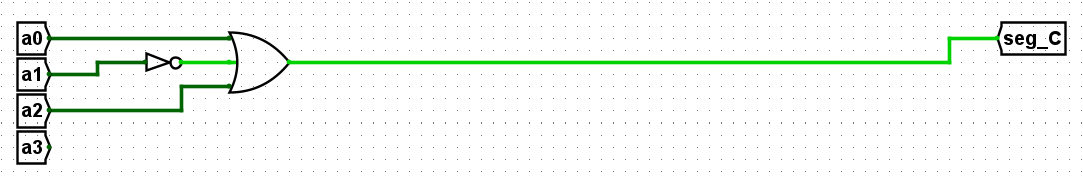
\includegraphics[width=1\textwidth]{segment_C.png}
    \caption{Logikschaltung Segment C}
    \label{fig:segment_C}
\end{figure}

Die Logikschaltung zum Segment C wurde wie in Abbildung~\ref{fig:segment_C} gezeigt aufgebaut.

% ----------------- Tabelle -----------------
\vspace{1em} % Abstand
Nachfolgend die Wahrheitstabelle der Segmente:
\begin{table}[ht]
\centering
\colorlet{BFH-table}{BFH-MediumBlue!10}
\colorlet{BFH-tablehead}{BFH-MediumBlue!50}
\setupBfhTabular
\begin{bfhTabular}{llllllllllll}
Input & a3 & a2 & a1 & a0 & seg\_A & seg\_B & seg\_C & seg\_D & seg\_E & seg\_F & seg\_G \\\hline
\num{0} & \num{0} & \num{0} & \num{0} & \num{0} & \num{1} & \num{1} & \num{1} & \num{1} & \num{1} & \num{1} & \num{0} \\\hline
\num{1} & \num{0} & \num{0} & \num{0} & \num{1} & \num{0} & \num{1} & \num{1} & \num{0} & \num{0} & \num{0} & \num{0} \\\hline
\end{bfhTabular}
\caption{Wahrheitstabelle Siebensegmentanzeige}
\label{tab:truthtable_bcd_to_7segment}
\end{table}

%----------------  Results   -----------------------------------------------
\clearpage
\section{Resultate}
\section{Results}
What did you find? – a section which describes the data that was collected and the results of any statistical tests that were performed.  It may also be prefaced by a description of the analysis procedure that was used. If there were multiple experiments, then each experiment may require a separate Results section.

%----------------  Discussion   --------------------------------------------
\clearpage
\section{Diskussion}
Ziel des Abschnitts Diskussion ist es die Ergebnisse des Versuchs zusammenzufassen und zu reflektieren.
–	Erreichte Funktionalität und verbleibende Probleme
–	Fazit und Reflexion

%----------------  Bibliography   ------------------------------------------
\clearpage
\printbibliography

%----------------  List of figures   ---------------------------------------
\clearpage
\listoffigures
 
%----------------  List of tables   ----------------------------------------
\clearpage
\listoftables

%----------------  List of listings   --------------------------------------
%\clearpage
%\lstlistoflistings 

%----------------  Glossary and acronyms  ----------------------------------
\clearpage
\printglossary[type=main]
\printglossary[type=acronym]

%------------ Index ----------------------
\clearpage
\printindex

%------------ Appendix ----------------	
\appendix
%\chapter{First Appendix Chapter}

\end{document}
